\begin{figure}[htbp]
    \centering
    \begin{minipage}{0.49\textwidth}
        \centering
        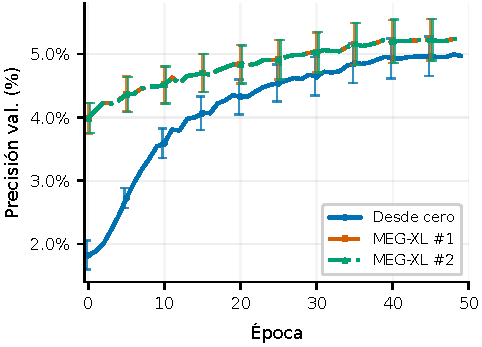
\includegraphics[width=\linewidth]{figuras/fig_5_1a_pretraining_reading_val_accuracy.pdf}
        \vspace{-0.5em}
        \centerline{\small (a) Lectura}
    \end{minipage}
    \hfill
    \begin{minipage}{0.49\textwidth}
        \centering
        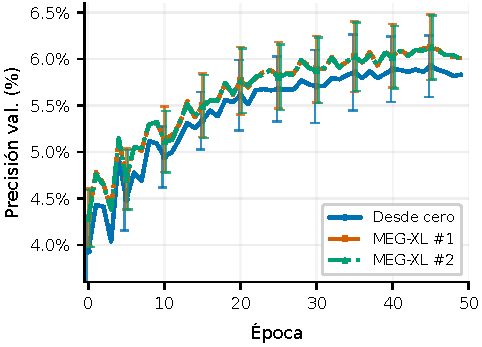
\includegraphics[width=\linewidth]{figuras/fig_5_1b_pretraining_listening_val_accuracy.pdf}
        \vspace{-0.5em}
        \centerline{\small (b) Escucha}
    \end{minipage}
    \caption[Precisión de validación durante el preentrenamiento autosupervisado]{Precisión de validación durante las dos etapas del preentrenamiento autosupervisado. La etapa de escucha continúa desde el checkpoint seleccionado tras la etapa de lectura para cada condición. Las barras de error, mostradas cada cinco épocas, indican una desviación típica entre los seis cuantizadores del tokenizador.}
    \label{fig:pretraining_val_accuracy}
\end{figure}
